


\chapter{Theory}
\label{chapter:theory}

\section{Protocol Attacks: TCP SYN Flooding}

TCP (Transmission Control Protocol) is one of the most common protocols within the transport layer, and one of the core of the Internet Protocol suite (IP). TCP provides reliable, ordered, error-checked of stream of packets between two hosts. In addition to these characteristics, TCP is a connection-oriented protocol, that is, a prior connection between both parties is necessary before starting the exchange of information. This process is known as TCP three-way handshake (Figure \ref{fig:TCPHandshake}).

\par

Suppose \textit{X} as a client that wants to carry out a friendly TCP connection with the server \textit{Y}. First of all, \textit{X} requests by sending a synchronize \textit{(SYN)} message to \textit{Y}. The server receives the request and responses by sending an acknowledge \textit{(SYN-ACK)} back to the client. Once the client receives the SYN-ACK, it responses with an ACK, an the connection is established. 

\par

While the server waits for the \textit{SYN-ACK's} response, it keeps the connection in a half open state and maintains a backlog queue for the information about the connections. Once the server receives the \textit{ACK}, it changes the state to \textit{established} and frees up memory of the queue. Because the size of the backlog queue is not infinite, the half-open connection will remain on it until a time-out is exceeded. In the case that the queue is full, all new incoming connection requests will be dropped.

\bigskip

\textbf{TCP SYN Flooding attack}, as suggested by the name, aims to exhaust the server's backlog queue flooding it with \textit{SYN} messages, but once they receive the corresponding \textit{SYN-ACK} from the server, they will not response with the \textit{acknowledge} message, forcing the server to keep the connection information in the backlog queue until the time-out is exceeded (Figure \ref{fig:SYNFlooding}). As a result, when a \textit{friendly} client wants to set up a TCP connection with the server, will be denied. The biggest challenge of the attacker is ensure that the source IP address which is used to establish the connection is not reachable by the server. Otherwise, the source will send a \textit{RST} packet to the server that cause server to reset the connection and free up the memory of the queue.


\begin{figure}[htb]
	\centering
	\subfigure[TCP Tree-way handshake]{%
		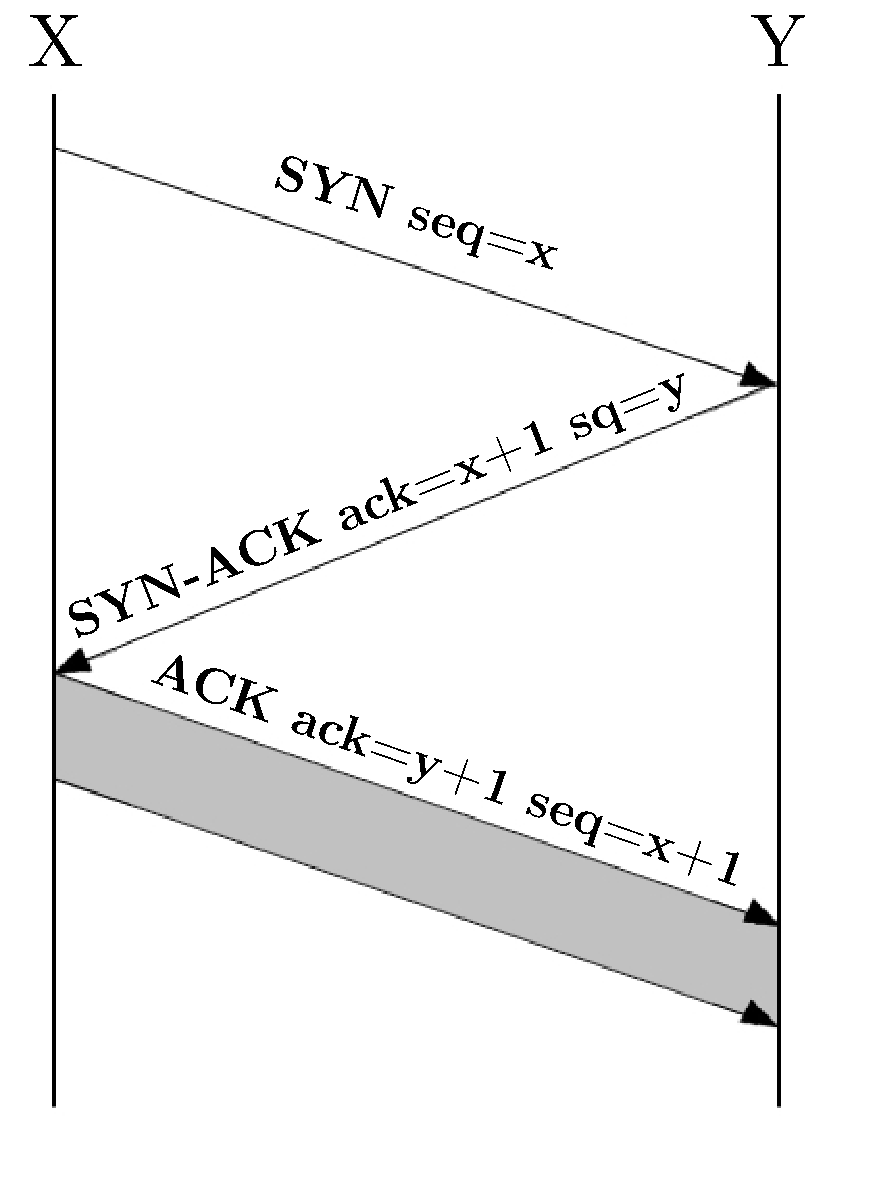
\includegraphics[width=0.5\textwidth]{./images/TCPHandshake.pdf}%
		\label{fig:TCPHandshake}%
	}%
	\hfill
	\subfigure[SYN Flooding]{%
		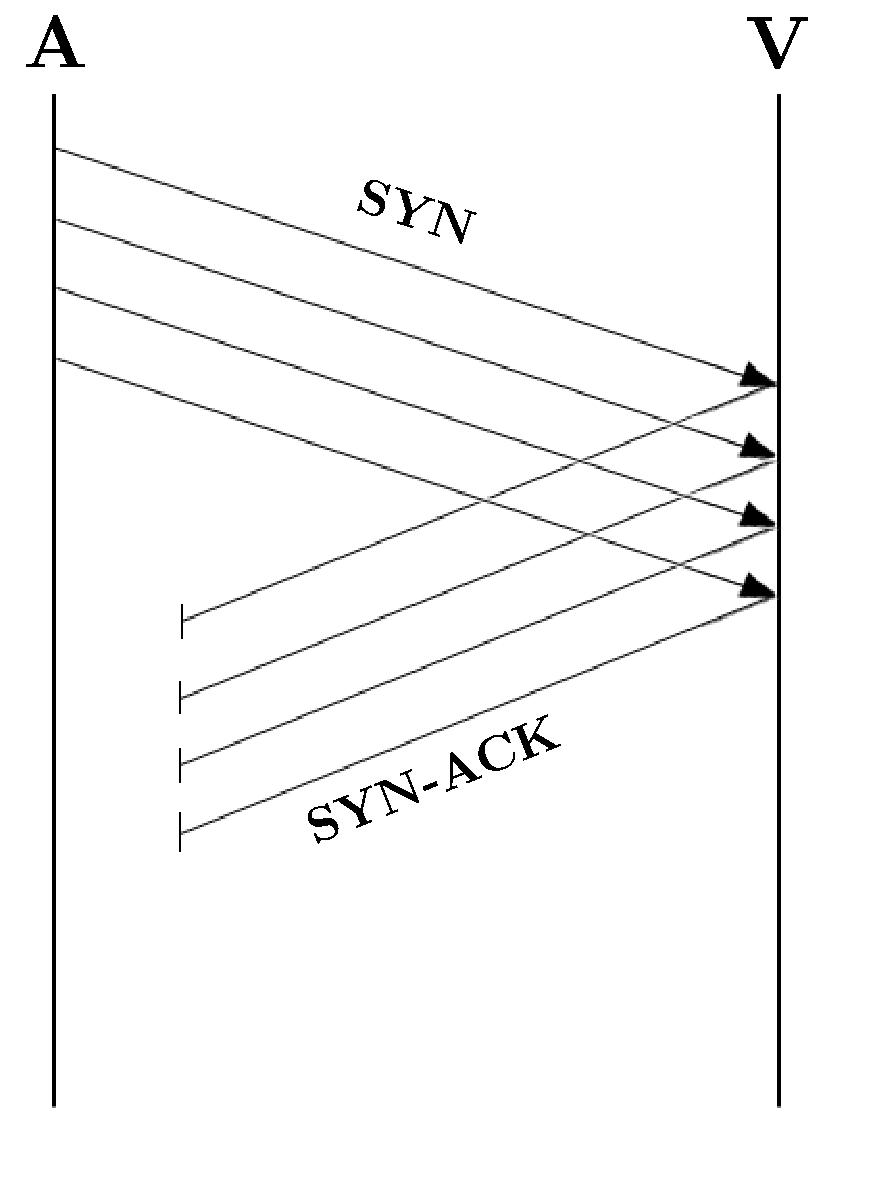
\includegraphics[width=0.5\textwidth]{./images/TCPSynAttak.pdf}%
		\label{fig:SYNFlooding}%
	}%
	\caption{TCP Three-way handshake and SYN Flooding} 
	\label{fig:TCPConnections}
\end{figure}



\subsection{Methods of Attack}
\label{subsec:SYNMethodsOfAttacks}

The attack can be categorized depending on how the attacker carries out the attack over the victim: Direct Attack, Spoofed-based Attack and Distributed Attack ~\cite{CiscoTCPSYN}.


\subsubsection{Direct Attack (Figure \ref{fig:DirectAttackSYN}) }
\label{subsec:SYNDirectAttack}

\begin{figure}[H]
\centering
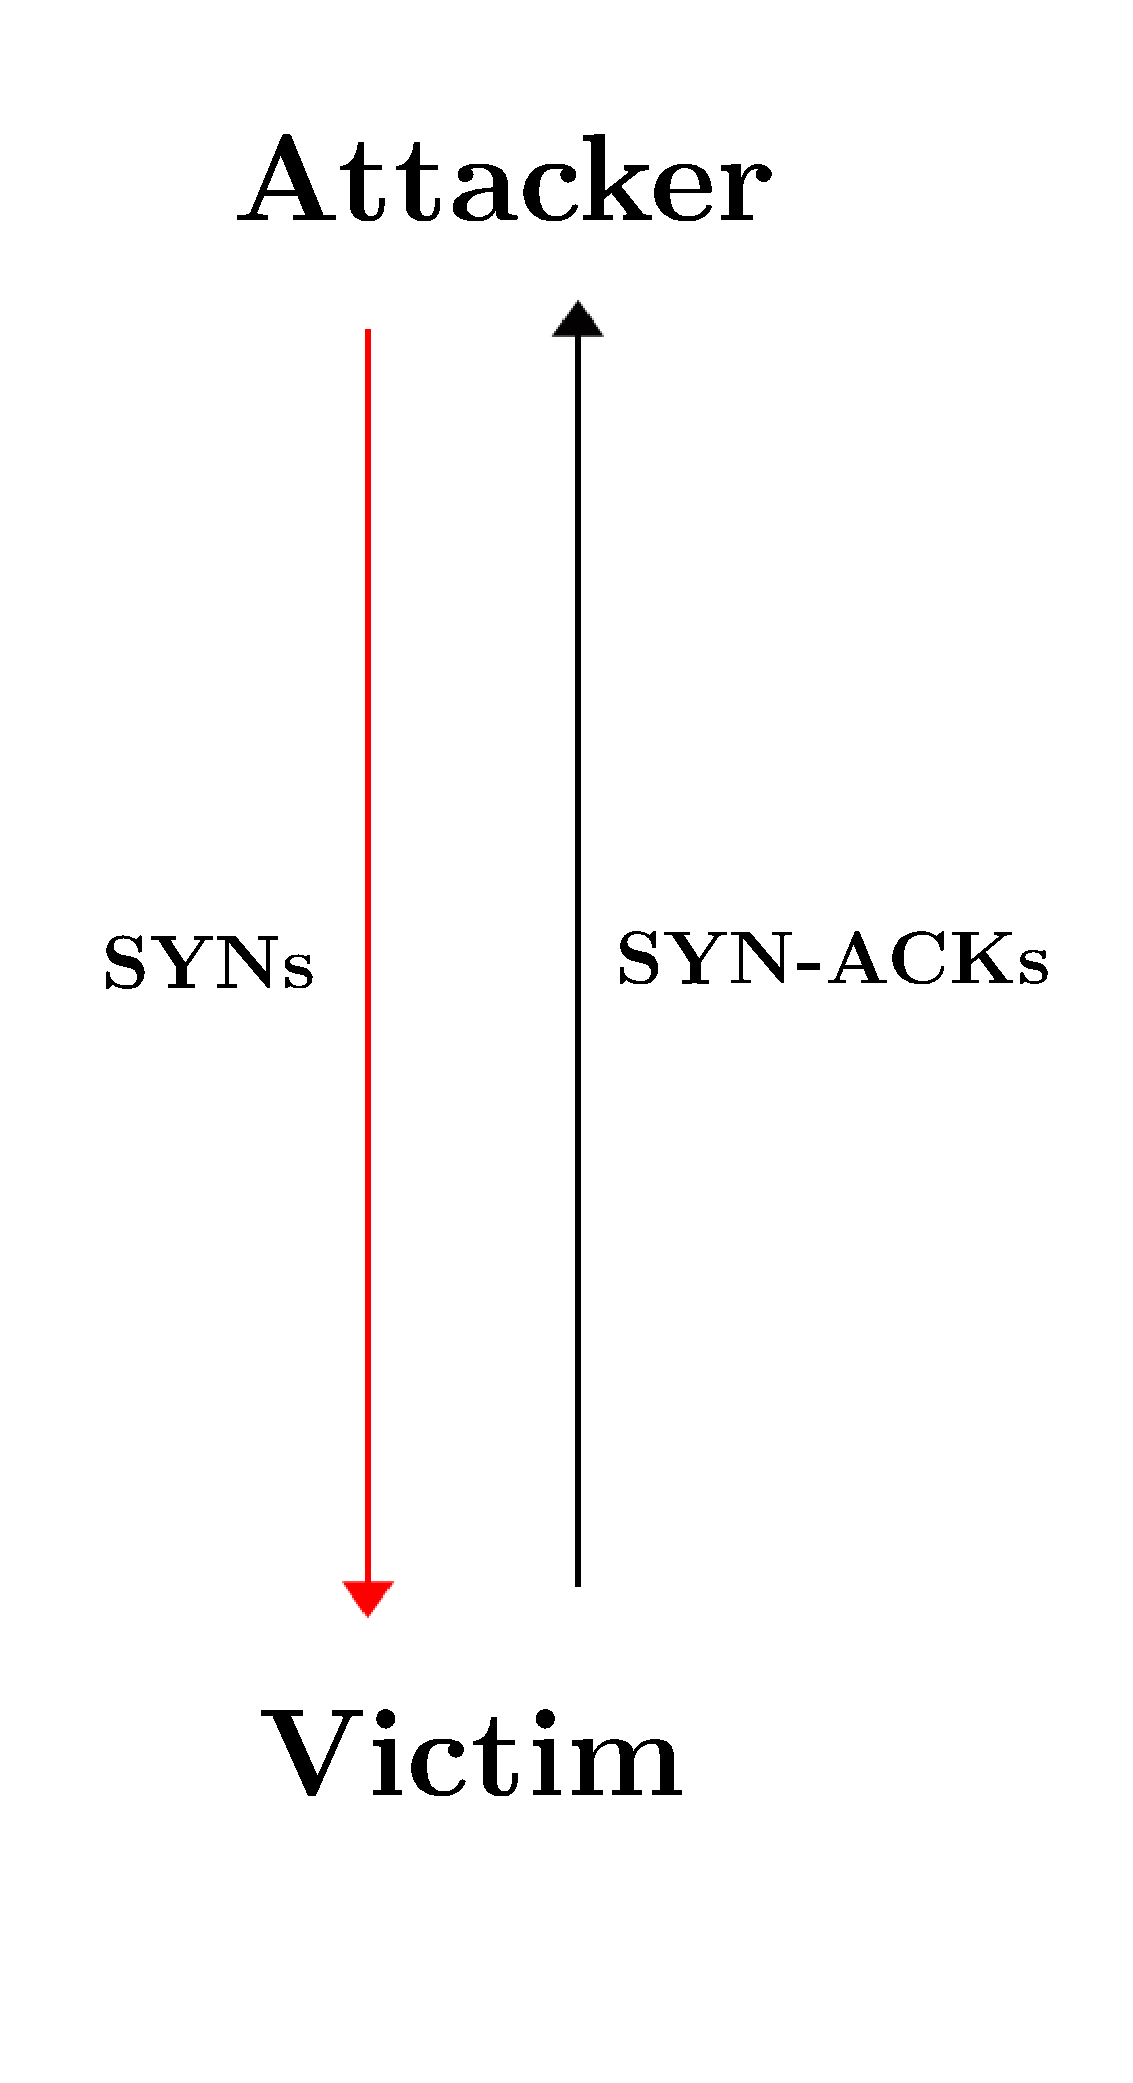
\includegraphics[height=0.4\textwidth]{./images/DirectAttackSYN.pdf}
\caption{Direct Attack} \label{fig:DirectAttackSYN}
\end{figure}

In this case, the attacker is the one that accomplishes the attack direct to the victim. It does not even spoof the source IP address. Instead, it will just ensures that there will not be response after it receives the \textit{SYN-ACK} message.

\subsubsection{Spoofed-based Attack (Figure \ref{fig:SpoofedAttackSYN})}
\label{subsec:SYNSpoofedAttack}

\begin{figure}[H]
\centering
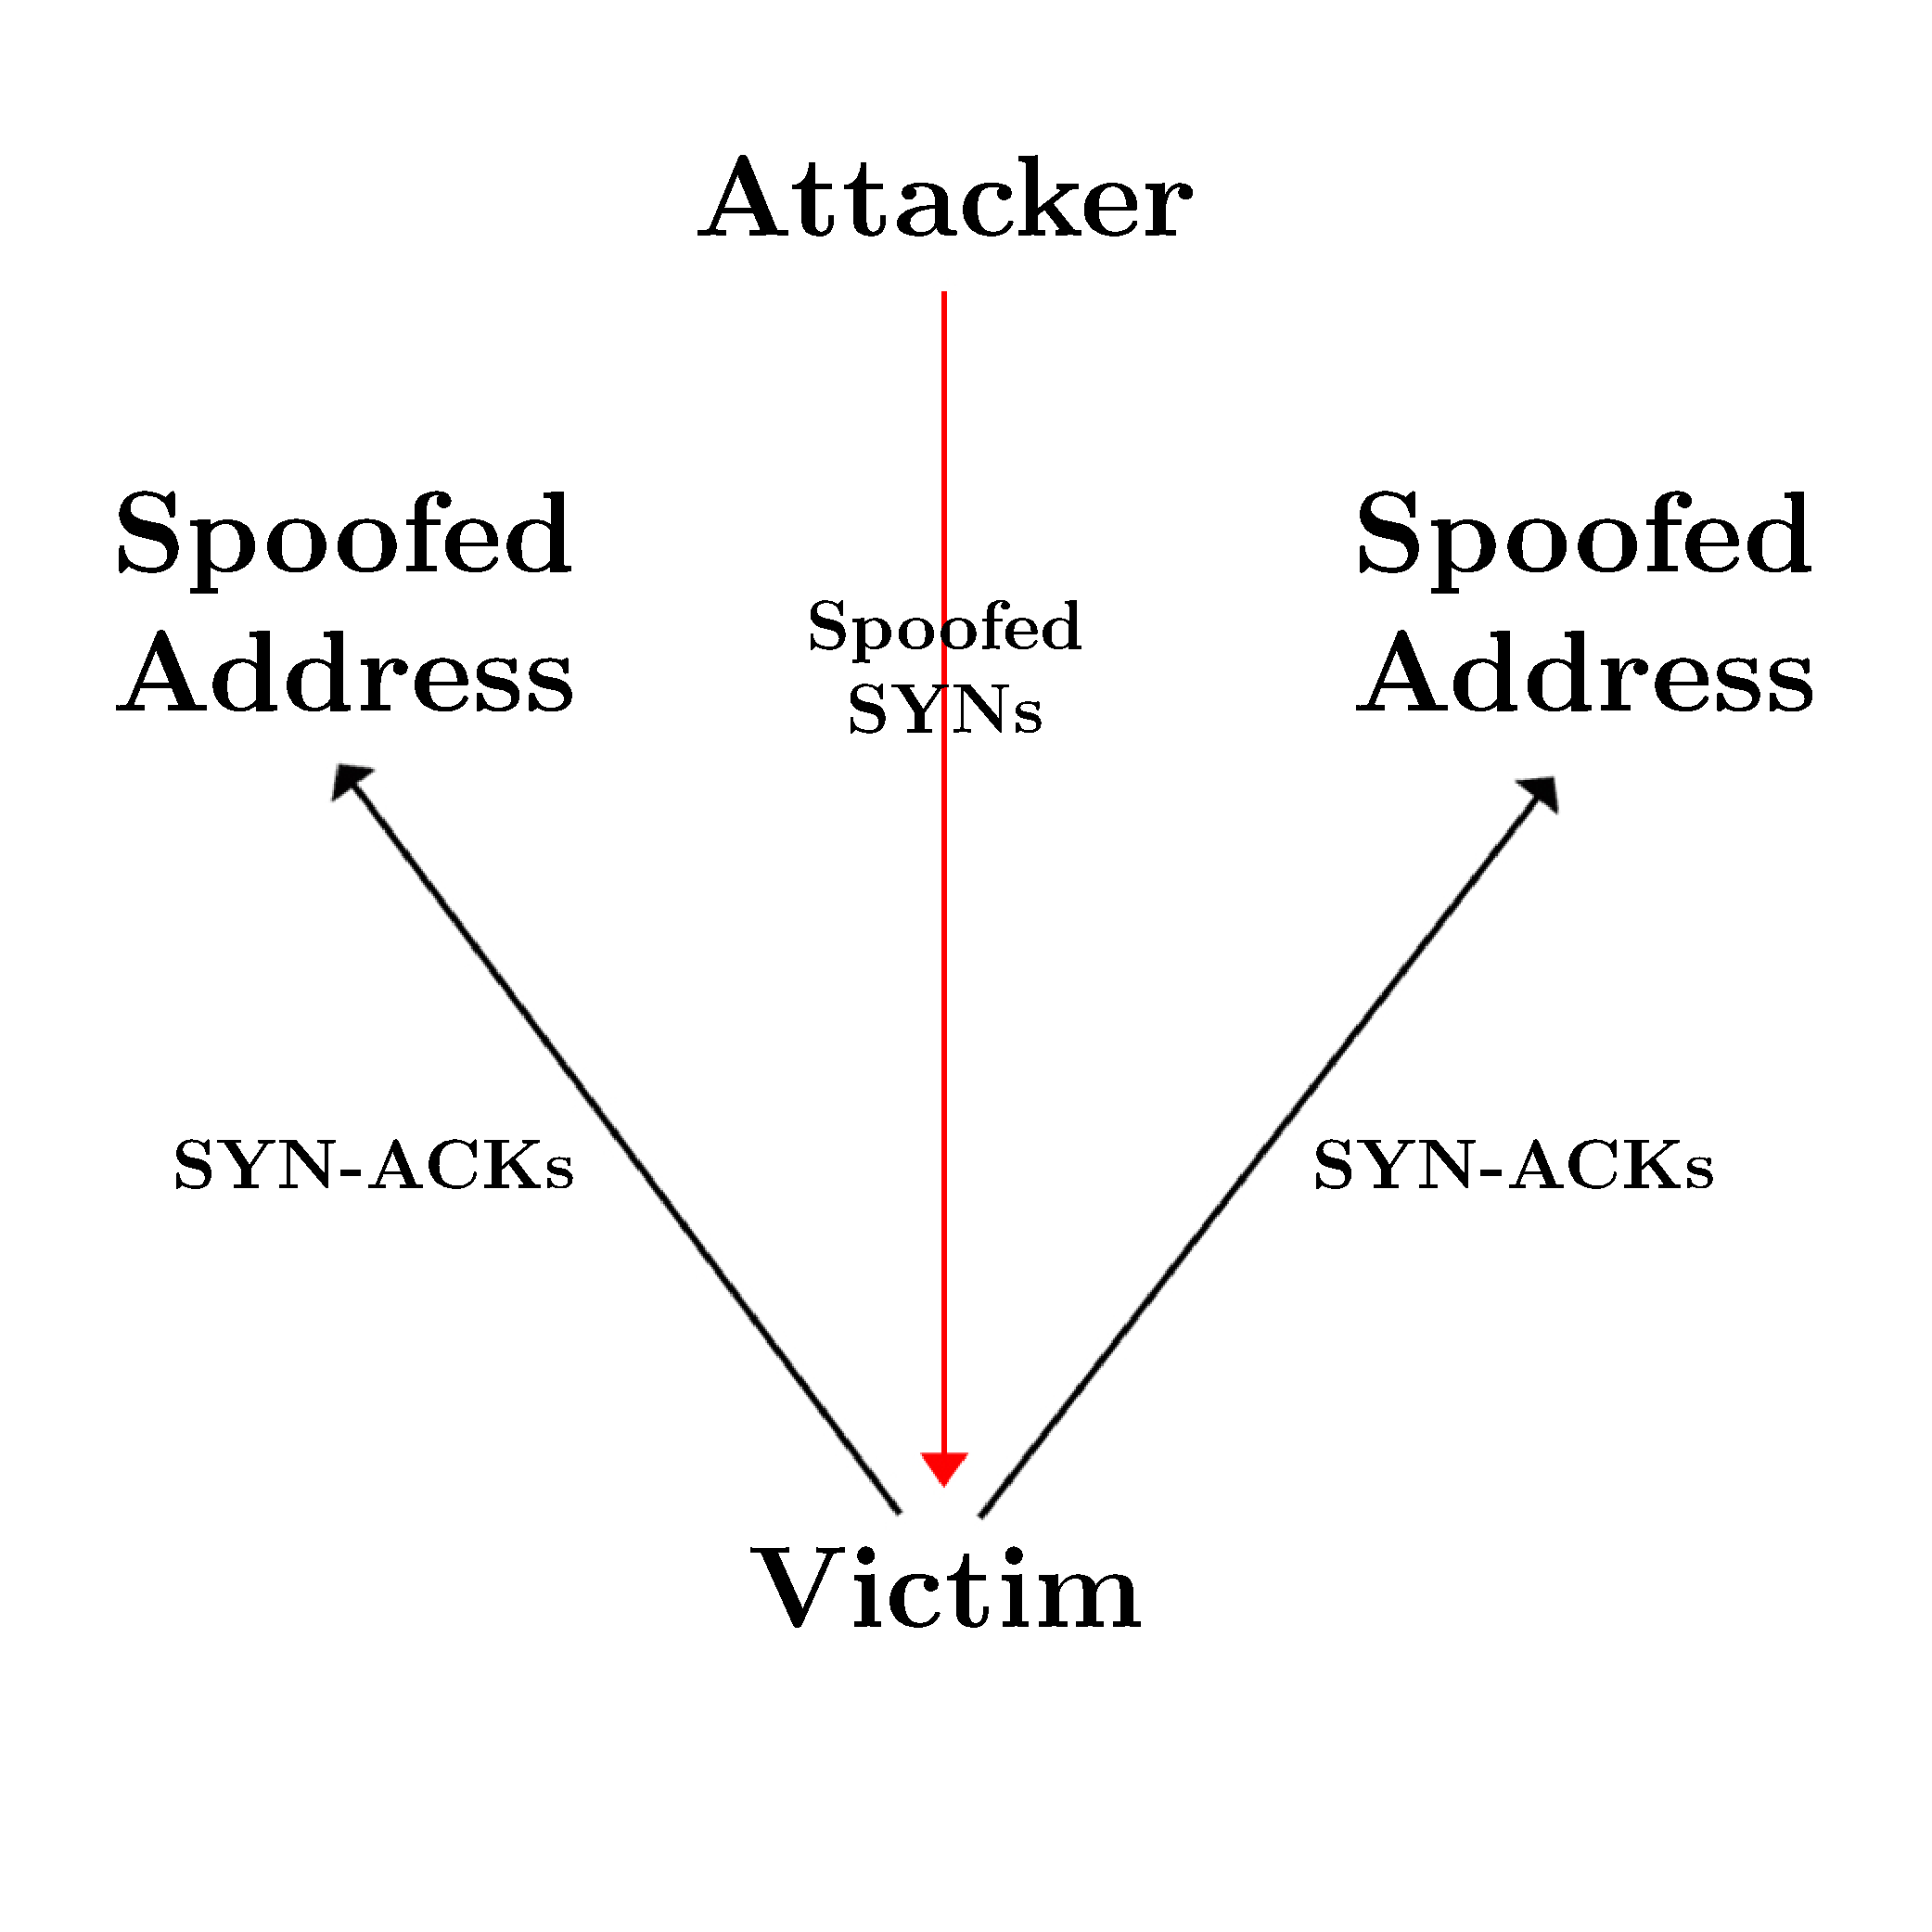
\includegraphics[width=0.4\textwidth]{./images/SpoofedAttackSYN.pdf}
\caption{Spoofed-based Attack} \label{fig:SpoofedAttackSYN}
\end{figure}

This version of SYN flooding attack direct to the victim, but it spoofs the source IP address in the \textit{SYN} packet. As we have explained before, a primary consideration is address selection. An attacker can choose spoofed IP address either using a single source which is known that will not response the \textit{SYN-ACK}, or using a list of source address under the assumption that some percentage of them will not response.


\subsubsection{Distributed Attack (Figure \ref{fig:DistributedAttackSYN})}
\label{subsec:SYNDistributedAttack}

\begin{figure}[H]
\centering
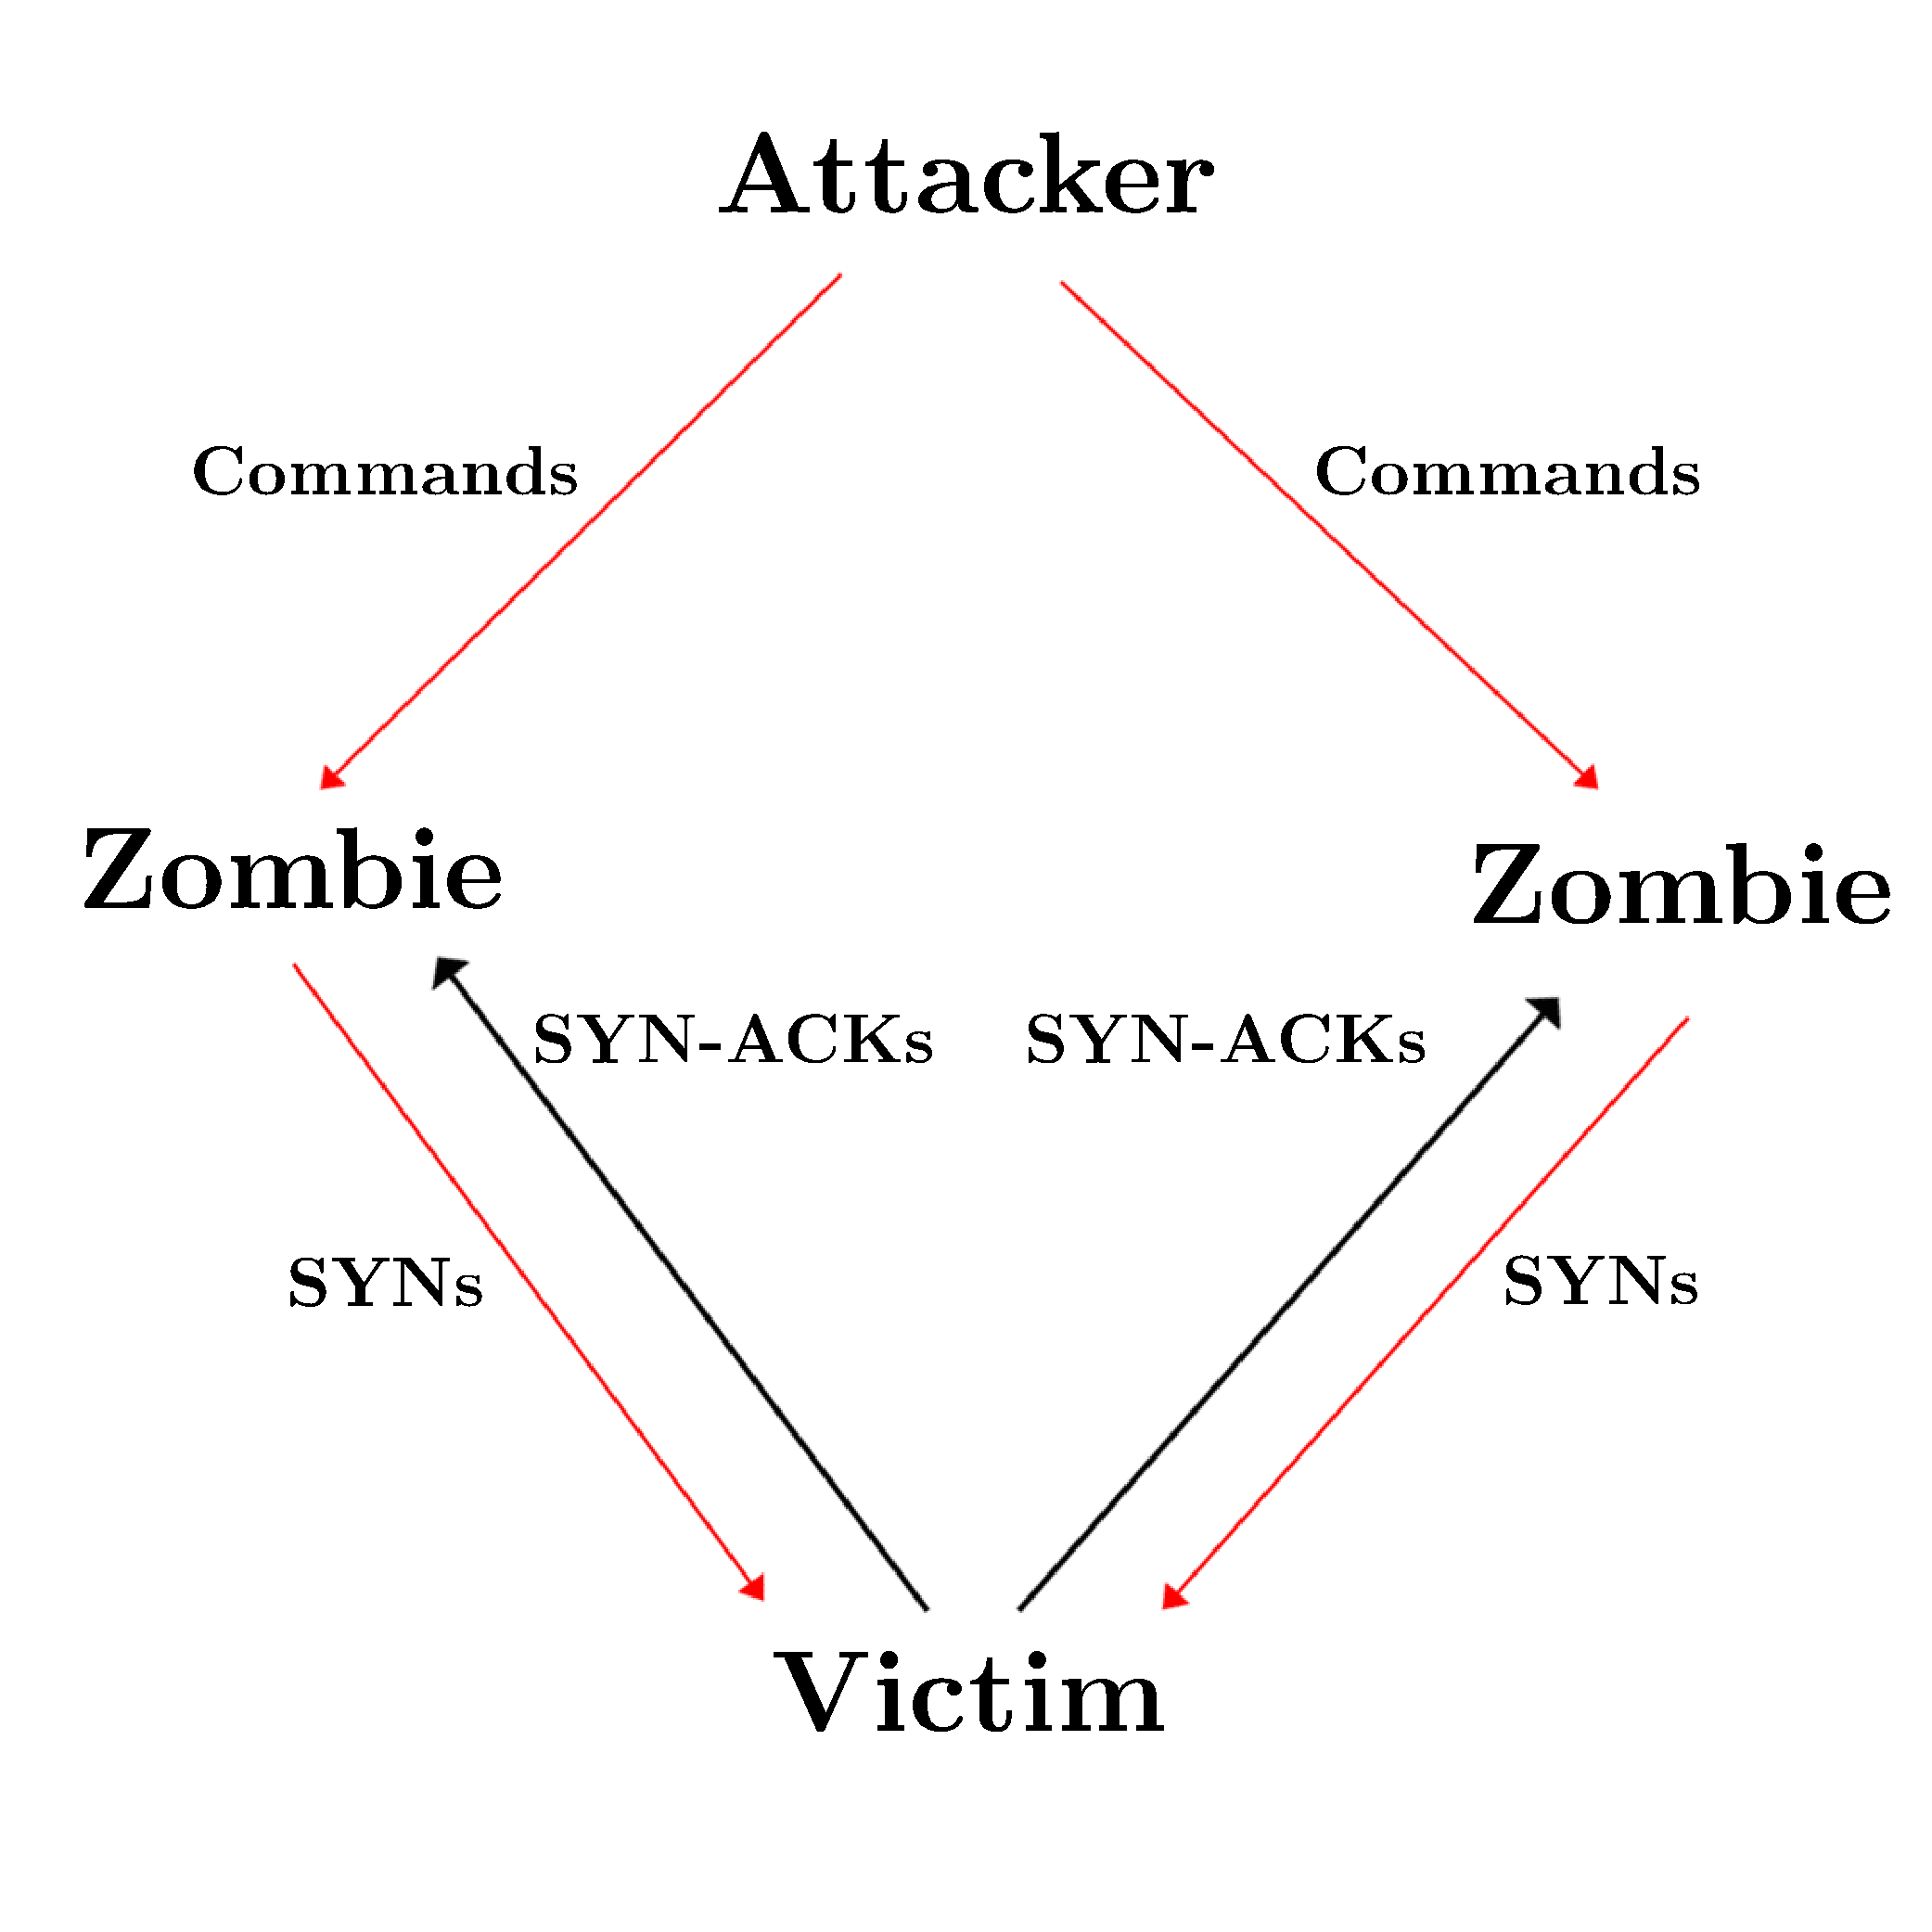
\includegraphics[width=0.4\textwidth]{./images/DistributedAttackSYN.pdf}
\caption{Distributed Attack} \label{fig:DistributedAttackSYN}
\end{figure}

In this case, the attacker carries out the attack through numerous zombie machines in internet. This attack is much more difficult to counter, due to the attacker is not the one that accomplish the attack. Zombie machines are constantly added and removed from the botnet.


\subsection{Prevention and Response}

Explain host-end defense and network defense. We will use network defense.

\subsection{TCP FLOODING DEFENSE PROPOSED (DRAFT!!!!)}

Hi Aapo, this is an another idea that I have thought using anomaly detection. Basically, I will implement two different kinds of anomaly detection, one to control the amount of traffic and the other filtering the headers of the packets to check if they have something unusual (IP header length, TCP payload, TCP TTL...). Also there will be implemented a Rate-Limiting filter, using a "delay-queue". I will try to explain you the main idea by steps below:\\

If the amount of traffic is usual, the router will follow the flow traffic as usual to the server but the Controller will store the IPs address that complete the three handshake connection in a "working set"(for future connection if an attack is detected).\\

Once the anomaly detection system detects that the traffic is bigger than a boundary or is increasing rapidly, it will be launch the defense mechanism, installing a flow match in the flow table that all the TCP SYN packets that arrive to the switch, will be send them to the Controller.\\

The scope of the controller is as follow:\\

First, it will match the incoming IP address with the "working set", if so, two flows in either directions between the internal host and the remote host will be set in the flow table. If it does not match, the other anomaly detection system will filter the headers of the packet (There is a survey that I have attached in the email that explain this algorithm, but you can see it in the Figure \ref{fig:AlgorithmAnomalyDetection}). It might happen:\\

1. If everything is OK, the request connection will be enqueue in the delay-queue (to control the rate of the incoming connections). Every \textit{d} seconds a new connection will be moved from the queue to the switch to forward it to the server. Whenever a positive connection reply, the IP address will be store in the "working set" and the new flow entries will be set in the flow table.\\

2. If some anomaly in the packet is detected, the IP address will be store in a "suspect IP addresses table". Here I am not sure what can I do yet, either drop the packet or the switch can send the SYN-ACK back, and if it response, a new flow entry will be set in the flow table.\\

I know that the packet header filtering will not find all the attacks, but at least a big part of them. The main idea is that the server will receive the traffic in a fixed rate and not whole the traffic that arrive to the network.\\

\begin{figure}[H]
\centering
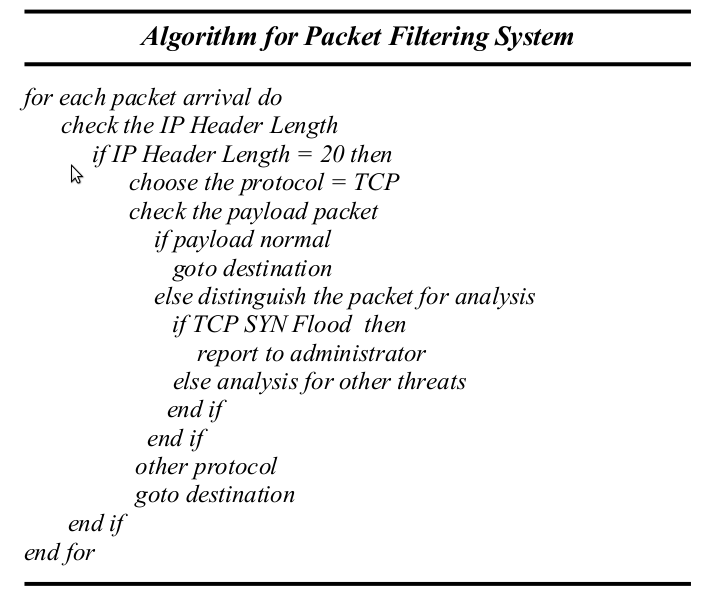
\includegraphics[width=1\textwidth]{./images/AlgorithmAnomalyDetection.png}
\caption{Packet Filtering Algorithm} \label{fig:AlgorithmAnomalyDetection}
\end{figure}

